\documentclass[solutions.tex]{subfiles}

\xtitle

\begin{document}
\maketitle
\begin{exercise} Consider the points $(x=\dfrac\pi2,\,y=-\dfrac\pi2)$,
$(x=-\dfrac\pi2,\,y=\dfrac\pi2)$, $(x=-\dfrac\pi2,\,y=-\dfrac\pi2)$.
Are these points stationary points of the following functions? If so,
of what type?
\begin{equation*} \begin{aligned}
	F(x,y) &&=\quad& \sin x + \sin y \\
	G(x,y) &&=\quad& \cos x + \cos y
\end{aligned} \end{equation*}
\end{exercise}
\begin{remark} We've renamed the second function from $F$ to $G$
for clarity: we're going to work them both at once, as the process
(and the functions) are very similar.
\end{remark}

To get an idea, of what we could expect, we can start by plotting
those functions, on a range containing those points:
\begin{figure}[H]
	\centering
	\begin{minipage}{0.45\textwidth}
		\centering
		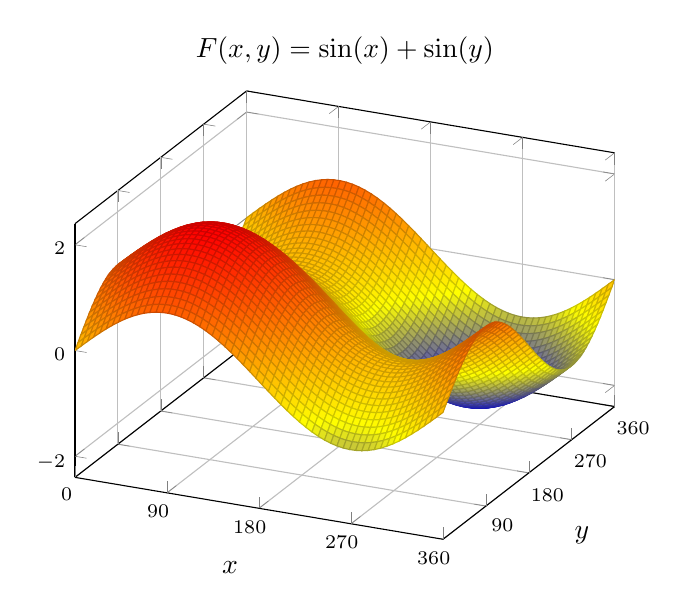
\begin{tikzpicture}
			\begin{axis} [
			    title = {$F(x,y) = \sin(x)+\sin(y)$},
			    xtick = {0,90,...,360},
			    ytick = {90,180,...,360},
			    xlabel = $x$, ylabel = $y$,
			    ticklabel style = {font = \scriptsize},
				grid
			]
			\addplot3 [surf, domain=0:360, samples=60]
				{ sin(x)+sin(y) };
			\end{axis}
		\end{tikzpicture}
	\end{minipage}
	\begin{minipage}{0.45\textwidth}
		\centering
		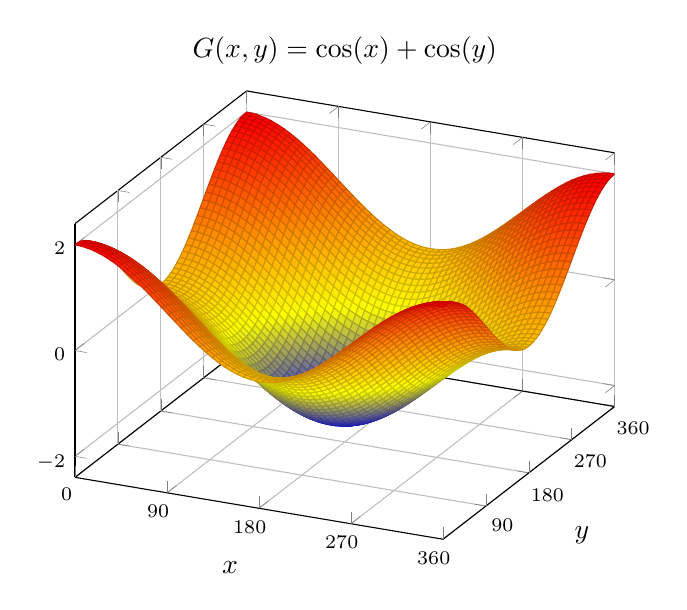
\begin{tikzpicture}
			\begin{axis} [
			    title = {$G(x,y) = \cos(x)+\cos(y)$},
			    xtick = {0,90,...,360},
			    ytick = {90,180,...,360},
			    xlabel = $x$, ylabel = $y$,
			    ticklabel style = {font = \scriptsize},
				grid
			]
			\addplot3 [surf, domain=0:360, samples=60]
				{ cos(x)+cos(y) };
			\end{axis}
		\end{tikzpicture}
	\end{minipage}
\end{figure}

% TODO: display gradians instead of degrees; highlights our
% points of interest:
% https://tex.stackexchange.com/questions/320629/how-to-draw-in-tikz-with-label-in-radians

For $F$, we seem to have:
\begin{itemize}
	\item a local maximum at $(\dfrac\pi2,\dfrac\pi2)$ (not asked);
	\item a local minimum at $(-\dfrac\pi2,-\dfrac\pi2)$;
	\item two saddles at $(\dfrac\pi2,-\dfrac\pi2)$ and $(-\dfrac\pi2,\dfrac\pi2)$.
\end{itemize}

And for $G$, $(\pi,\pi)$ seems to be a minimum (not asked); all other points don't
seem to be much of interests. It seems we have some maximums on the corners
(e.g. $(0,0)$), and perhaps some saddle points in between, but not only the graph
isn't complete enough to tell, and we're not asked about those points anyway.

\hrr

Analytically, this requires us first to determine if those points are
stationary, and then to compute  all the second order derivatives
for both functions, so as to apply the second partial derivative test.
Let's start by computing all the derivatives we'll need:

\begin{equation*} \begin{aligned}
	F_x(x,y) &&=\quad& \cos x; &&\quad&
		G_x(x,y) &&=\quad& -\sin x \\
	F_y(x,y) &&=\quad& \cos y; &&\quad&
		G_y(x,y) &&=\quad& -\sin y \\
	F_{x,x}(x,y) &&=\quad& -\sin x; &&\quad&
		G_{x,x}(x,y) &&=\quad& -\cos x \\
	F_{y,y}(x,y) &&=\quad& -\sin y; &&\quad&
		G_{y,y}(x,y) &&=\quad& -\cos y \\
	F_{x,y}(x,y) &&=\quad& 0; &&\quad&
		G_{x,y}(x,y) &&=\quad& 0 \\
	F_{y,x}(x,y) &&=\quad& 0; &&\quad&
		G_{y,x}(x,y) &&=\quad& 0 \\
\end{aligned} \end{equation*}

\begin{remark} Remember that $\varphi_{x,y}$ means the second order derivative
obtained by first differentiating on $x$, then on $y$. Also remember that
by Clairaut's theorem\footnote{
\url{https://en.wikipedia.org/wiki/Symmetry\_of\_second\_derivatives}}, we
could have assumed, in the context of classical mechanics, the symmetry of
the second order derivatives; they are all really trivial to compute in
the present case.
\end{remark}

Let's recall the definition of Hessian matrix, wrapping the second
order derivatives of a scalar field $\Phi$:
\[
	\bm{H}_\Phi = \begin{pmatrix}
		\Phi_{x,x} & \Phi_{y,x} \\
		\Phi_{x,y} & \Phi_{y,y} \\
	\end{pmatrix}
\]

In our case, because the mixed derivatives are zero, it will
have the following form, both for $F$ and $G$:
\[
	\bm{H}_\Phi = \begin{pmatrix}
		\Phi_{x,x} & 0 \\
		0& \Phi_{y,y} \\
	\end{pmatrix}
\]
And so the determinant and trace will be, again for both $F$ and $G$:
\[
	Det(\bm{H}_\Phi) = \Phi_{x,x}\Phi_{y,y};\quad\quad
		Tr(\bm{H}_\Phi) = \Phi_{x,x}+\Phi_{y,y}
\]
Now, points are \textit{stationary} when all first-order derivatives
are zero at once. We can then determine whether they are local
minimum/maximum or saddle points using the second partial derivative test
\footnote{\url{https://en.wikipedia.org/wiki/Second\_partial\_derivative\_test}}:
\begin{itemize}
	\item $Det(\bm{H}_\Phi) > 0$ and $Tr(\bm{H}_\Phi) > 0$ : \textit{local minimum};
	\item $Det(\bm{H}_\Phi) > 0$ and $Tr(\bm{H}_\Phi) < 0$ : \textit{local maximum};
	\item $Det(\bm{H}_\Phi) < 0$: \textit{saddle};
	\item $Det(\bm{H}_\Phi) = 0$: inconclusive (this case isn't mentioned in the book).
\end{itemize}

\begingroup
	\renewcommand\arraystretch{1.5}
	\setlength\LTleft{-0.45in}
	\centering
    \addtolength{\leftskip} {-2cm} % increase (absolute) value if needed
%	\begin{longtable}{|@{} C{.125\textwidth} *{6}{C{.1\textwidth}} C{.125\textwidth} @{}|}
	\begin{longtable}{|@{} C{.1\textwidth} *{4}{C{.135\textwidth}} *{2}{C{.1\textwidth}} C{.13\textwidth} @{}|}
	\hline
	\textbf{P} & \textbf{$F_x=\cos x$} & \textbf{$F_y=\cos y$} & \textbf{$F_{x,x} = -\sin x$} & \textbf{$F_{y,y} = -\sin y$} &
		\textbf{$Det(\bm{H}_F)$} & \textbf{$Tr(\bm{H}_F)$} & \textbf{Type} \endhead \hline
		$(\dfrac\pi2,-\dfrac\pi2)$ & 0 & 0 & $-1$ & $1$ & $-1$ & $0$ & \textbf{saddle} \\
		$(-\dfrac\pi2,\dfrac\pi2)$ & 0 & 0 & $1$ & $-1$ & $-1$ & $0$ & \textbf{saddle} \\
		$(-\dfrac\pi2,-\dfrac\pi2)$ & 0 & 0 & $1$ & $1$ & $1$ & $2$ & \textbf{local minimum} \\
	\hline
	\end{longtable}
\endgroup

As far as $G$ is concerned:
\[
	x \in \{ \frac\pi2, -\frac\pi2\},\quad G_x(x,y) = -\sin(x) \Rightarrow G_x(x,y) \ne 0
\]
\[
	y \in \{ \frac\pi2, -\frac\pi2\},\quad G_y(x,y) = -\sin(y) \Rightarrow G_y(x,y) \ne 0
\]

That is to say, the first derivatives don't go to zero for any of those
points, hence none of them are stationary points for $G$ to begin with.

\end{document}
